\documentclass[12pt]{article}
\usepackage[utf8]{inputenc}
\usepackage{amsmath}
\usepackage{graphicx}
\begin{document}
\date{}
\section*{Reporte Producto 5: Descripción de actividades}

 En la actividad 5 se modificó un programa proporcionado por el profesor, de tal manera que nos arrojara datos como el alcance en los ejes "x" y "y", y el tiempo total de vuelo, graficando a su vez el tiro parabólico que se obtiene de introducir un ángulo y una velocidad inicial.
 A continuación se presentan los resultados de la práctica con sus respectivas descripciones.\\
 
\subsection*{Actividades realizadas y evidencias:}
 
Vas a tratar de reproducir los resultados que muestra la simulación de Phet, proporcionando la rapidez inicial y el ángulo de disparo, para encontrar en que punto cae al suelo el proyectil.\\
 Verifica la consistencia de tu programa, lanzando tu proyectil a 90º hacia arriba, a 0º, a 30º y 60º.
 Se verificó la efectividad del programa corriéndolo con distintos ángulos.\\
 Evidencias:\\
 \begin{verbatim}
   !************************************************  
  !This program plots projectile motion of an object.  
  !The program requires user input for initial velocity   
  !and angle of the object.The algorithm uses a time   
  !step of 0.01 second i.e. it calculates object's  
  !location in the x and y plane every 0.01 second.  
  !**********By: Waleed Ishaque, 2013**************  
  program projectile_plot  
       implicit none  
       !Defining constants:  
       real, parameter :: pi = 4.0*atan(1.0)
       real :: u, a, t, a_grados  
       real, parameter :: g = 9.81  
       real:: x(150),y(150)  
          integer :: i
!where g is gravity, pi is "pi"   
       !u is object's initial velocity   
       !a is object's initial angle   
       !t is time during the simulation   
       !x and y are arrays with 150 rows   
       !Seek user input   
       write(*,*) 'Enter angle of projectile (Real)'   
       read *, a_grados   
       write(*,*) 'Enter velocity of projectile (Real)'   
       read *, u   
       !Convert angle to radians   
       a = a_grados*pi/180.0   
       !open .dat file and start writing on it using the algorithm   
       open(1, file='proj.dat')   
       do i=1,100   
 !displacement of object in x and y direction   
            t = (float(i)*0.01)   
            x(i) = u*cos(a)*t   
           y(i) = u*sin(a)*t - 0.5*g*t*t   
  !write output in file "proj.dat" for plotting   
            \end{verbatim}
            \centering
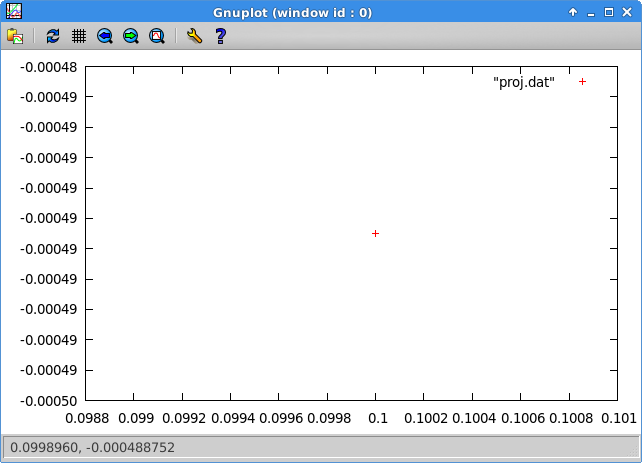
\includegraphics[scale=0.5]{0.png}

            \newpage
 

 \centering
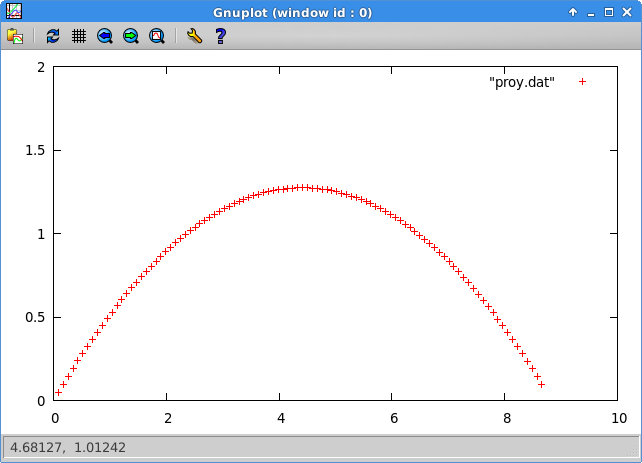
\includegraphics[scale=0.5]{30.png}

 

 \centering
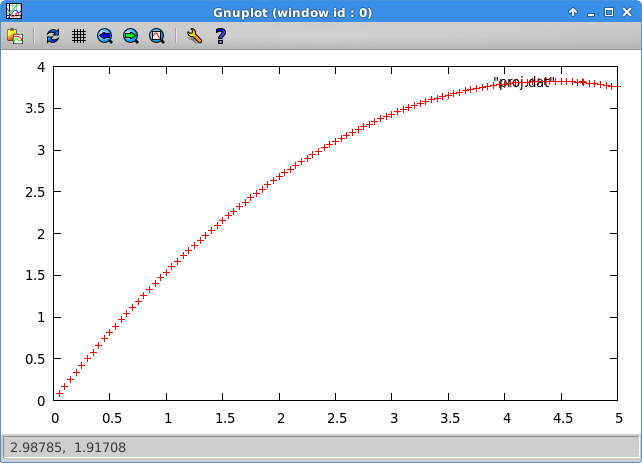
\includegraphics[scale=0.5]{60.png}

 
 


 \centering
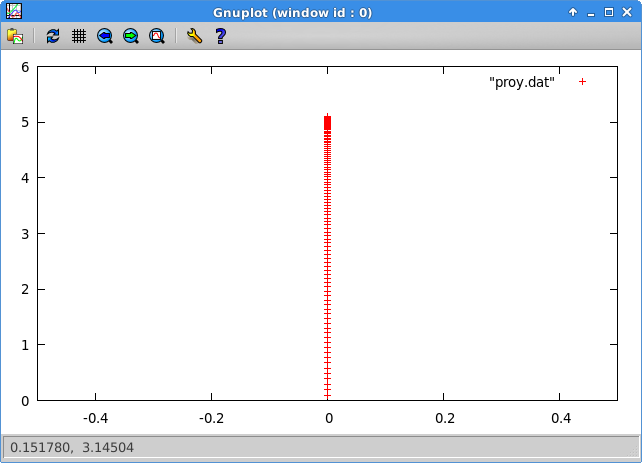
\includegraphics[scale=0.5]{90.png}


 \newpage
 Se pide incluir el cálculo del tiempo total de vuelo T, la altura máxma H que alcanza, y el alcance máximo R del proyectil. (Ver ecuaciones del proyectil en Wikipedia).
 Se modificó el prorgrama en emacs para que nos arrojara estos datos, de talmanera que al correr el programa aparecieran como variables.\\
 
 \begin{verbatim}
 Program proyectil_2
implicit none
real, parameter :: pi = 4.0*atan(1.0)
real :: v, a, t, h, r, a_grados
real, parameter :: g = 9.81
real :: x(150),y(150)
integer :: i
write (*,*) 'Introduzca un ángulo'
read *, a_grados
write (*,*) 'Ingrese una velocidad inicial'
read *, v
a = a_grados*pi/180.0
t = 2*v*sin(a)*(1/g)
h = v*v*sin(a)*sin(a)*(1/(2*g))
r = v*v*sin(2*a)*(1/g)
print * , 'Tiempo total de vuelo=' , t
print * , 'Altura máxima alcanzada=' , h
print * , 'Distancia máxima alcanzada=' , r
open(1, file='proy.dat')
do i=1,100
t = (float(i)*0.01)
x(i) = v*cos(a)*t
y(i) = v*sin(a)*t - 0.5*g*t*t
write(1,*) x(i), y(i)
if (y(i)<0) exit
end do
close(1)
End Program proyectil_2
 \end{verbatim}
 


 \centering
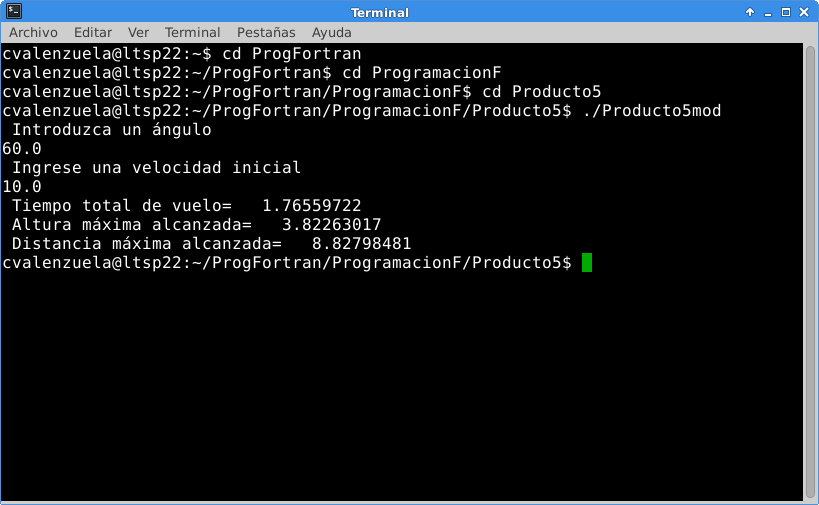
\includegraphics[scale=0.5]{Evidencias.png}

\end{document}

